\documentclass[UTF8]{ctexart}

\usepackage{subfiles}  

%下面的语句, 引入你的头部设置文件
\usepackage{C:/phpStorm_proj/02_myself_ID_EGO/+100_latex_all_math_sel/myPreamble} 
%必须是绝对路径,才能让各个tex在单独编译时使用到

\title{文件名}


%---------------------------------


\begin{document}
	\tableofcontents % 生成目录
	\date{} % 若不写这句, 则默认也会渲染出日期, 所以我们要手动赋空值
	\maketitle  %这行代码, 让你前面的 title, author, date生效
	
	
	\section{离散型 : 二项分布 (binomial distribution) : \\ B(试验次数n, 单次成功概率p)}
	
		
	
	\textbf{二项, 代表``有两个结果". 比如, 一个为``成功", 另一个为``失败".} \\	
	
	- 如: 投硬币10次(而不是只做一次实验),让X 代表``正面向上的次数”. 那么X 就是一个服从``二项分布"的随机变量 --- 每投一次硬币只有两种结果: 要么是"正面朝上", 要么是"反面朝上". \\
	- 你的教授给来了一个惊喜的突击测验,考试是10个判断题. 你对某一道题的猜测, 就属于``伯努利事件 a Binomial Event"  (因为它只有两种选择, "对"或"错"). 而整个测验(连续做n次伯努利事件), 是属于一个``二项事件" the entire quiz is a Binomial Event. \\
	
	所以\textbf{本质上,``二项事件"是一系列相同的``伯努利事件".} \\
	
	我们用字母``B”来表示二项分布, 即: $\boxed{B(\text{试验次数}n, \text{每项试验成功的概率}p)}$. \\
	
	\begin{myEnvSample}
		如: 我们将 $X \sim B(10, 0.6)$ 读作: 变量X 遵循10次试验中, 每项试验成功的可能性为0.6的 二项分布. \\
		Variable “X” follows a Binomial distribution with 10 trials /and a likelihood of success of 0.6 /on each individual trial. 
	\end{myEnvSample}

	\textbf{二项分布表示, 在特定的次数内, 能达到我们``期望结果"的可能性.} the graph of the binomial distribution /represents(v.) the likelihood of /attaining(v.) our desired outcome /a specific number of times. \\


某事件A发生的概率是P, 我们在做了n次试验后, 得到``该事件A 发生了k次", 则: 
\begin{align*}  % 支持每行编号. 若不需要编号, 就用 align*环境
	&P\left( X=k \right) =\underset{\text{总}n\text{中取}k}{\underbrace{C_{n}^{k}}}\cdot \underset{k\text{次成功}}{\underbrace{P^k}}\cdot \underset{n-k\text{次失败}}{\underbrace{\left( 1-P \right) ^{n-k}}}\ \ \ k=0,1,2,...,n.\\
&\text{记作:}X \sim B\left( \underset{\text{一共做了}n\text{次实验}}{\underbrace{n}},\underset{\text{事件}A\text{发生的概率}}{\underbrace{p}} \right)
\end{align*}
\vspace{1em} 

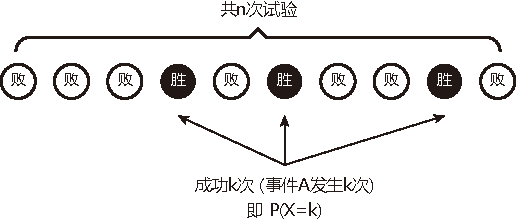
\includegraphics[width=0.65\textwidth]{/0145.pdf} \\



\begin{myEnvSample}
某药物, 临床有效率为0.95. 今有10人服用, 问``至少有8人能治愈"的概率是多少? (即做10次实验, 8次成功) \\
代入``二项分布"公式:
\begin{align*}  % 支持每行编号. 若不需要编号, 就用 align*环境
	P\left( X\ge 8 \right) 
&=\underset{}{\underbrace{P\left( X=8 \right) }}+\underset{}{\underbrace{P\left( X=9 \right) }}+\underset{}{\underbrace{P\left( X=10 \right) }}\\
&=\underset{P\left( X=8 \right)}{\underbrace{C_{10}^{8}\cdot 0.95^8\cdot \left( 1-0.95 \right) ^2}}+\underset{P\left( X=9 \right)}{\underbrace{C_{10}^{9}\cdot 0.95^9\cdot \left( 1-0.95 \right) ^1}}+\underset{P\left( X=10 \right)}{\underbrace{C_{10}^{10}\cdot 0.95^{10}\cdot \left( 1-0.95 \right) ^0}}\\
&=0.0746348+0.315125+0.598737 \\
&=0.988496
\end{align*}

所以, 10人中有8人以上被治愈的概率, 为0.98. \\

- geogebra 中的用法: \\
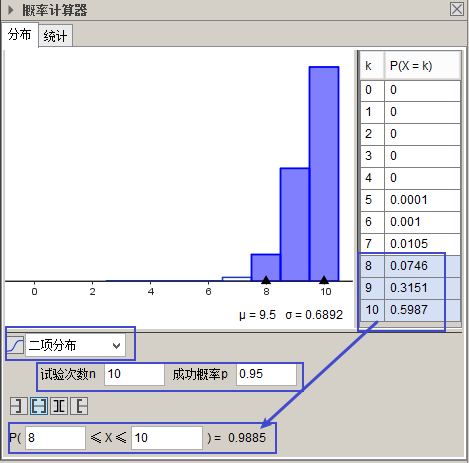
\includegraphics[width=0.7\textwidth]{/0138.png} \\

上表中, P(X=8)=0.0746 的意思, 就是 (对于单次实验是0.95的成功率的事件,) ``做10次实验, 里面会成功8次" 的概率=7.46\%. \\
同理, P(X=9) 的意思, 是``做10次实验, 里面会成功9次" 的概率. \\

- mathematica 中的用法: \\
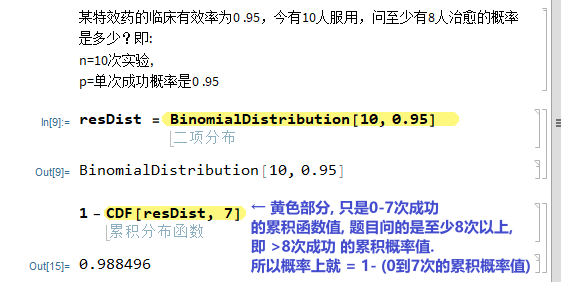
\includegraphics[width=0.8\textwidth]{/0139.png} \\

\textbf{即: 我们只要知道单次的成功概率, 就能计算n次成功中, 会成功k次的概率. }
\end{myEnvSample}
\vspace{1em} 



\begin{myEnvSample}
	某报警器, 在发生危险时, 成功报警的概率是0.8. 问: 要将报警成功率提高到99\%, 至少要安装多少台才行? \\
	我们令: \\
	- n: 表示总共安装的台数. \\
	- X: 表示成功报警的台数. \\	
	则, 安装的总n台中, 只要至少有一台能报警 (即 $P(X \geq 1)$), 就成功了. \\
	
	本例即: $X \sim B (\text{一共做n次实验},\text{单次实验的成功概率}0.8)$ 	
	\begin{align*}  % 支持每行编号. 若不需要编号, 就用 align*环境
	&\text{即:\ }\underset{\text{至少1台报警\ 的概率}}{\underbrace{P\left( X\ge 1 \right) }}\ge 0.99\\
&\underset{\text{全都没报警\ 的概率}}{\underbrace{1-P\left( X=0 \right) }}\ge 0.99\\
&1-\underset{\text{总}n\text{台里面,只有0台报警}}{\underbrace{C_{n}^{0}\cdot \underset{0\text{台报警\ 的概率}}{\underbrace{0.8^0}}\cdot \underset{n\text{台没报警\ 的概率}}{\underbrace{0.2^n}}}\ge 0.99}\\
&1-0.2^n\ge 0.99\\
&1-0.99\ge 0.2^n\\
&\ln 0.01\ge \ln 0.2^n\ \gets \text{两边取}\ln\\
&\ln 0.01\ge n\ln 0.2\\
&n\leq \frac{\ln 0.01}{\ln 0.2}\\
&n\leq \frac{-4.60517}{-1.60944}\\
&n\geq 2.86135
	\end{align*}
	
	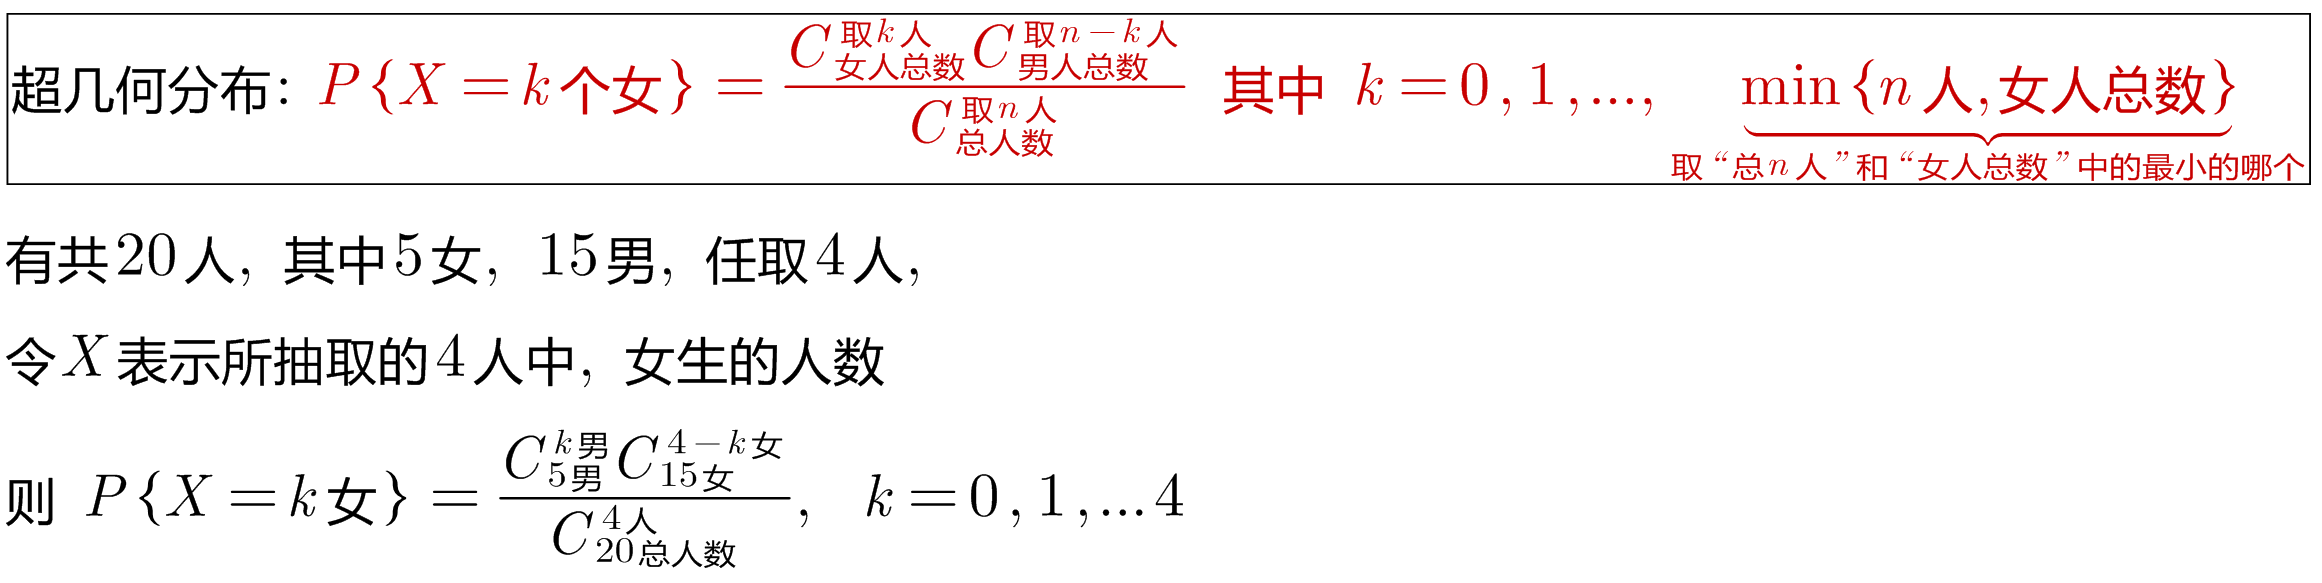
\includegraphics[width=0.6\textwidth]{/0140.png} \\
	
	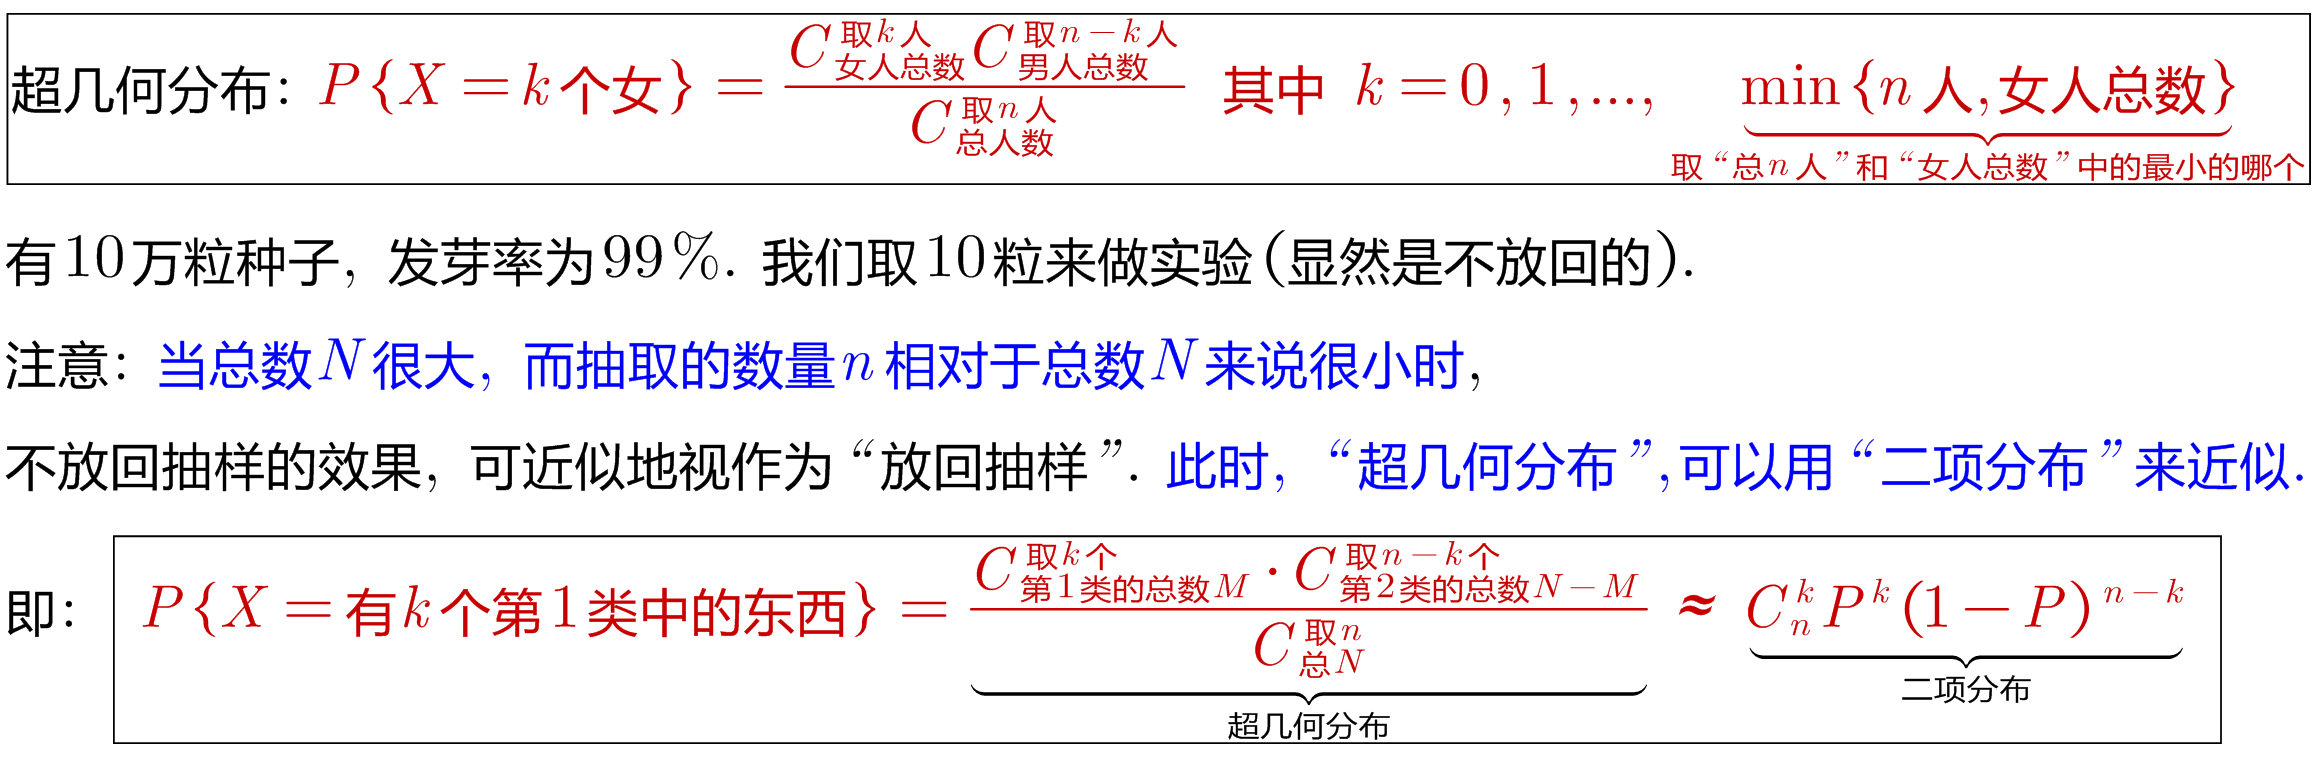
\includegraphics[width=0.6\textwidth]{/0141.png} \\
	
	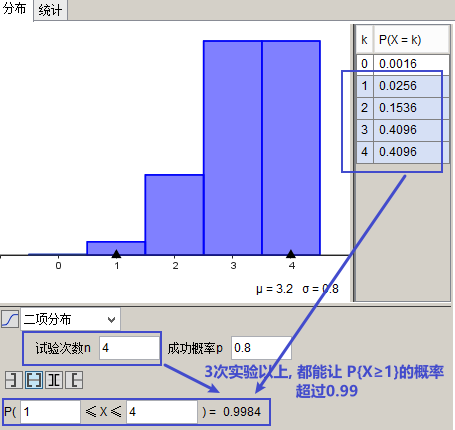
\includegraphics[width=0.6\textwidth]{/0142.png} \\
	

\end{myEnvSample}
\vspace{1em} 





\begin{myEnvSample}
	每台机器(机床), 会坏的概率是0.01. (即一台机器只有两种结果: 要么处在``正常工作"的状态, 要么处在``损坏"的状态.) 问: \\
	
	→ 若1个人(维修工)要看护20台机器. 他无法及时维修的概率是多少? 那么对1个人来说, 什么叫做``他无法及时维修"? 就是同时有 ≥ 2台机器处在``损坏"状态. \\
	我们令: \\
	- n: 代表总机器数. 本处 n=20. \\
	- 随机变量X: 表示``机器处在损坏状态"的台数. 即本处要求的就是 $P(X \geq 2)$ 的概率. 	
	\begin{align*}  % 支持每行编号. 若不需要编号, 就用 align*环境		
	&P\left( X\ge 2 \right) =1-P\left( X<2 \right)\\
&=1-\left[ \underset{\text{坏0台的概率}}{\underbrace{P\left( X=0 \right) }}+\underset{\text{坏1台的概率}}{\underbrace{P\left( X=1 \right) }} \right]\\
&=1-\left[ \left( \underset{0\text{台坏了,即全没坏}}{\underbrace{C_{20}^{0}}}\cdot \underset{\text{每台坏的概率}}{\underbrace{0.01}}^0\cdot \underset{\text{每台没坏的概率}}{\underbrace{0.99}}^{20-0} \right) +\left( \underset{20\text{台中坏了1台}}{\underbrace{C_{20}^{1}}}\cdot 0.01^1\cdot 0.99^{20-1} \right) \right]\\
&=0.0169
	\end{align*} 

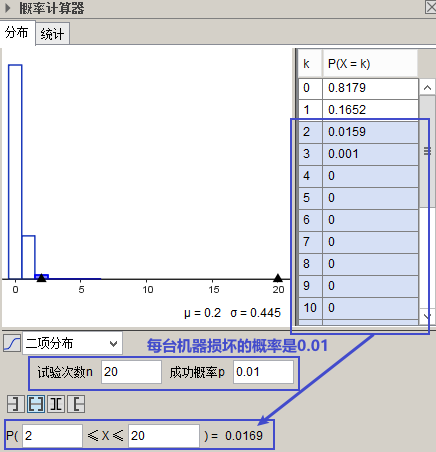
\includegraphics[width=0.65\textwidth]{/0143.png} \\


→ 若3个人看护80台机器, 问他们无法及时维修的概率?  那就是说, 同时有 ≥ 4台机器处在``损坏"状态. 即我们要求的是  $P(X \geq 4)$ 的概率. 
\begin{align*}  % 支持每行编号. 若不需要编号, 就用 align*环境
	&P\left( X\ge 4 \right) =1-P\left( X<4 \right)\\
&=1-\left[ \underset{\text{坏0台的概率}}{\underbrace{P\left( X=0 \right) }}+\underset{\text{坏1台的概率}}{\underbrace{P\left( X=1 \right) }}+\underset{\text{坏2台的概率}}{\underbrace{P\left( X=2 \right) }}+\underset{\text{坏3台的概率}}{\underbrace{P\left( X=3 \right) }} \right]\\
&=1-\left[ \left( C_{80}^{0}\cdot 0.01^0\cdot 0.99^{80} \right) +\left( C_{80}^{1}\cdot 0.01^1\cdot 0.99^{80-1} \right) +...+\left( C_{80}^{3}\cdot 0.01^3\cdot 0.99^{80-3} \right) \right]\\
&=0.0087
\end{align*}

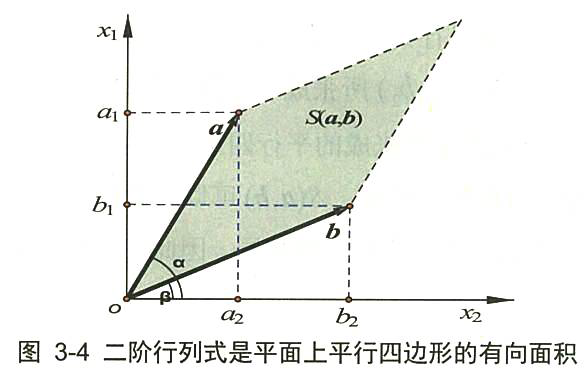
\includegraphics[width=0.65\textwidth]{/0144.png} 
\end{myEnvSample}
\vspace{1em} 


	
	\begin{tabular}{|p{0.4\textwidth}|p{0.6\textwidth}|}
		\hline
		 ``伯努利分布"(投1次硬币)的``期望值" E(Bernoulli event) &  就\textbf{表明我们对单个试验的预期结果.} the expected value of the Bernoulli distribution /suggests(v.) which outcome we expect for a single trial.\\
		\hline
		``二项分布"(投n次硬币)的``期望值" E(Binomial Event) &  是\textbf{我们期望获得特定结果的次数.} the expected value of the Binomial distribution /would suggest(v.) the number of times we expect to get a specific outcome. \\
		\hline
	\end{tabular}

	
	
	
\end{document}